\chapter{Prezentacja aplikacji}
Rozdział  został  poświęcony  prezentacji  zaimplementowanej  aplikacji webowej. Zrzuty ekranu zostały wykonane w przeglądarce Mozilla Firefox 70.0.1.
\section{Logowanie}
Na Rysunku \ref{fig:logowanie} przedstawiono ekran logowania. Jest to pierwsze co zobaczy użytkownik po uruchomieniu aplikacji. Aby przejść dalej należy podać prawidłowe dane logowania lub przejść do formularza rejestracji, aby założyć nowe konto.

\begin{figure}[H]
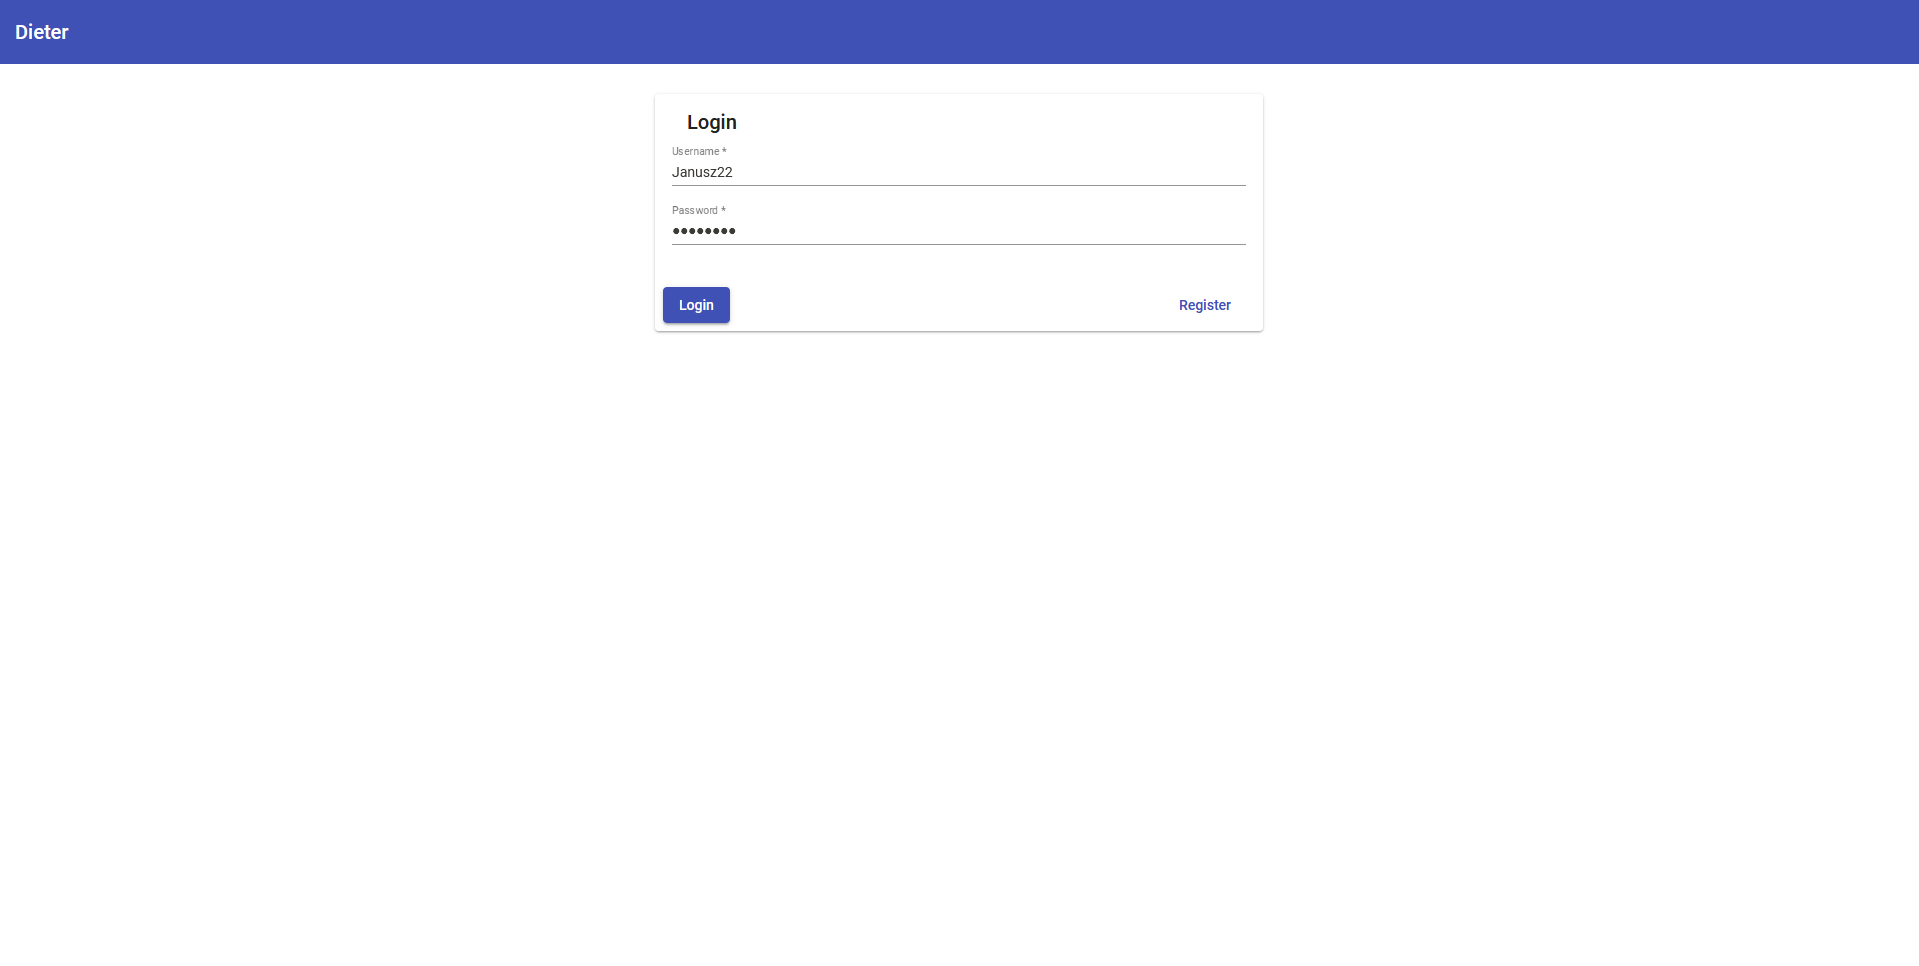
\includegraphics[width=\textwidth]{screeny/logowanie.png}
\caption{Ekran logowania}
\label{fig:logowanie}
\end{figure}

\section{Rejestracja}
Na Rysunku \ref{fig:rejestracja} przedstawiono formularz rejestracji. Aby się zarejestrować należy podać wszystkie wymagane dane w pola. Ich poprawność jest walidowana.

\begin{figure}[H]
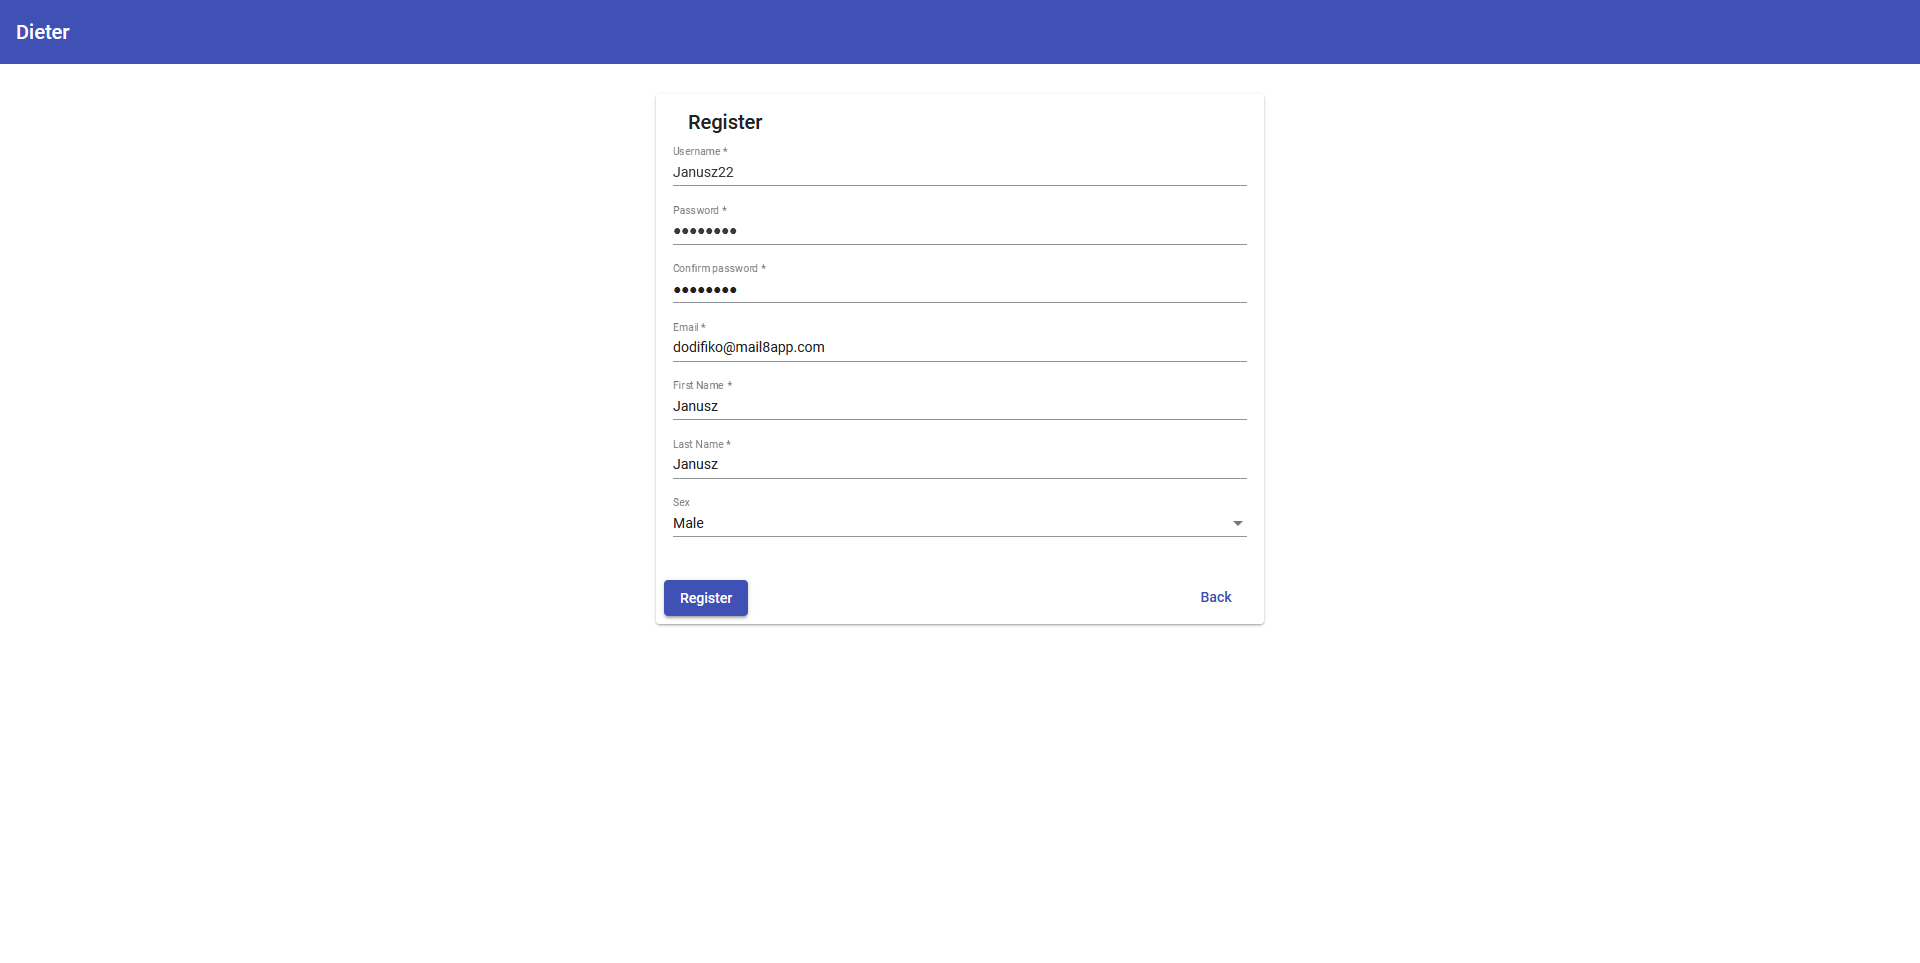
\includegraphics[width=\textwidth]{screeny/rejestracja.png}
\caption{Ekran rejestracji}
\label{fig:rejestracja}
\end{figure}

\section{Generowanie diety}
Na Rysunku \ref{fig:main} przedstawiono ekran generowania diety, a jednocześnie ekran główny aplikacji. Należy podać ilość posiłków, na które ma się składać dieta oraz średnie dzienne zapotrzebowanie kaloryczne. Efekt działania generatora można zobaczyć na Rysunku \ref{fig:use_case}. Po naciśnięciu w przepisu z listy wyświetlą się jego szczegóły. Natomiast po naciśnięciu przycisku \textit{Reset} można wygenerować nową dietę.

\begin{figure}[H]
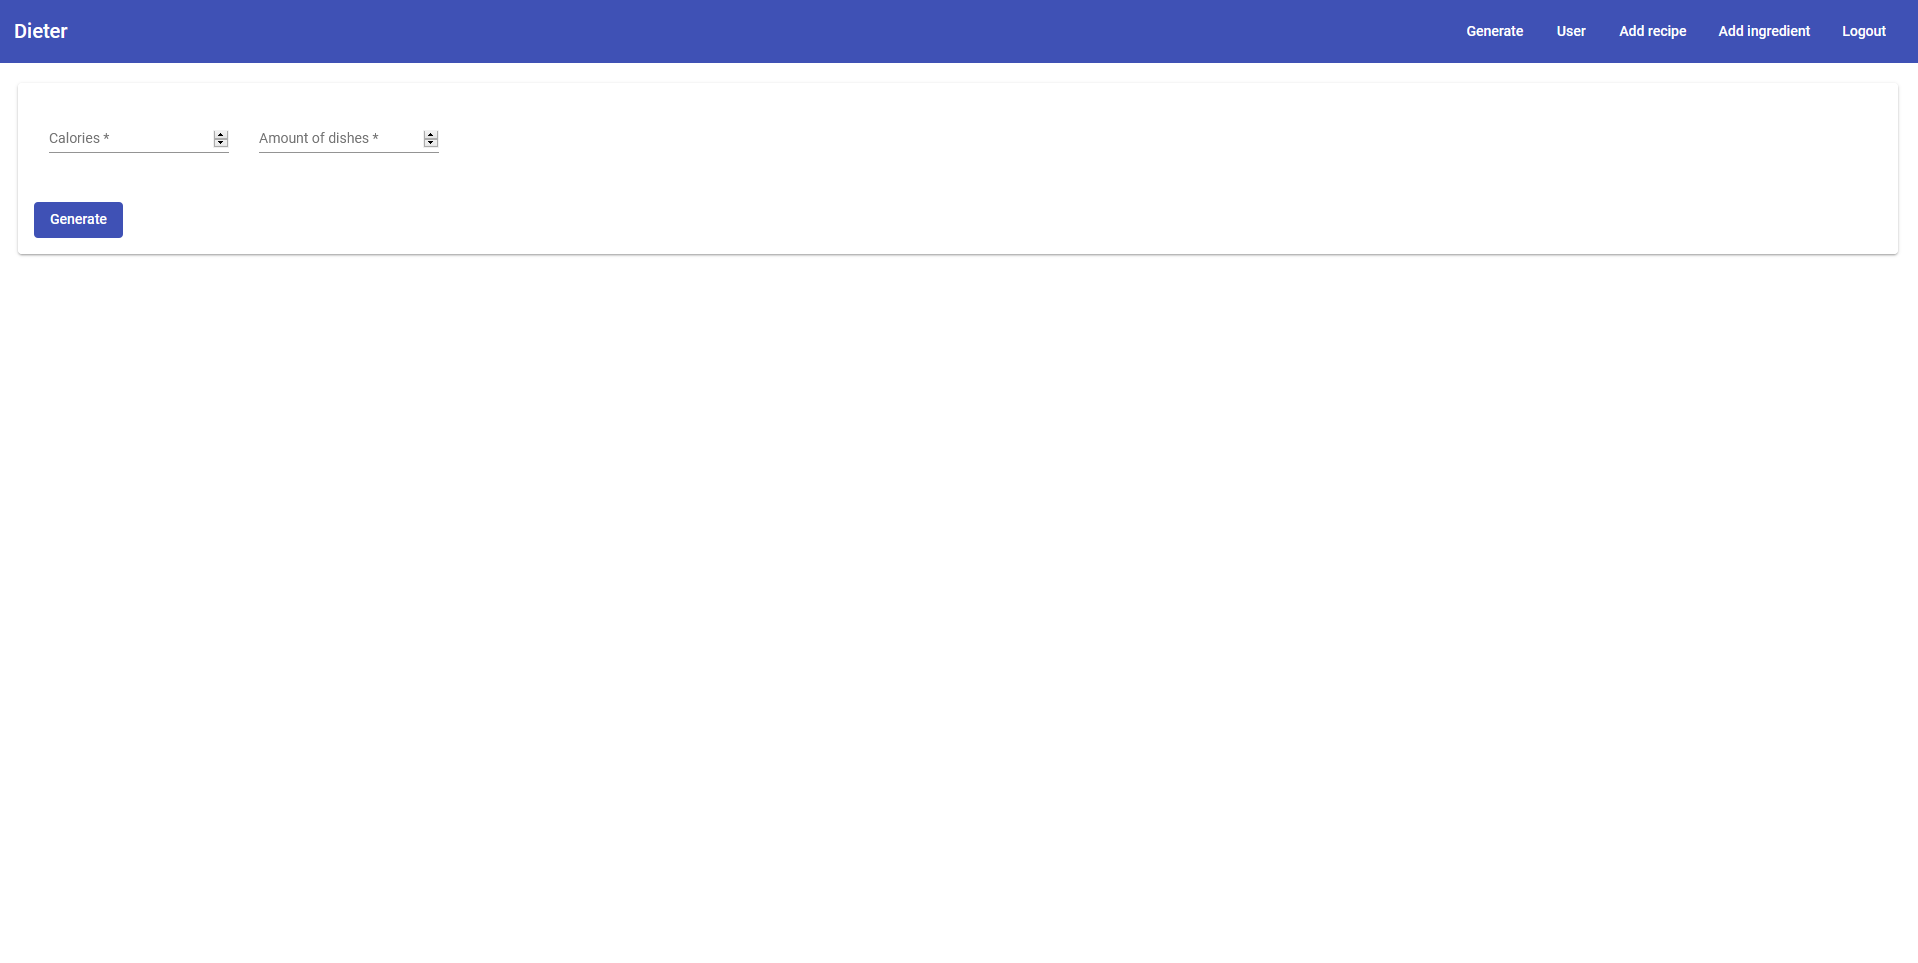
\includegraphics[width=\textwidth]{screeny/main.png}
\caption{Ekran główny}
\label{fig:main}
\end{figure}

\begin{figure}[H]
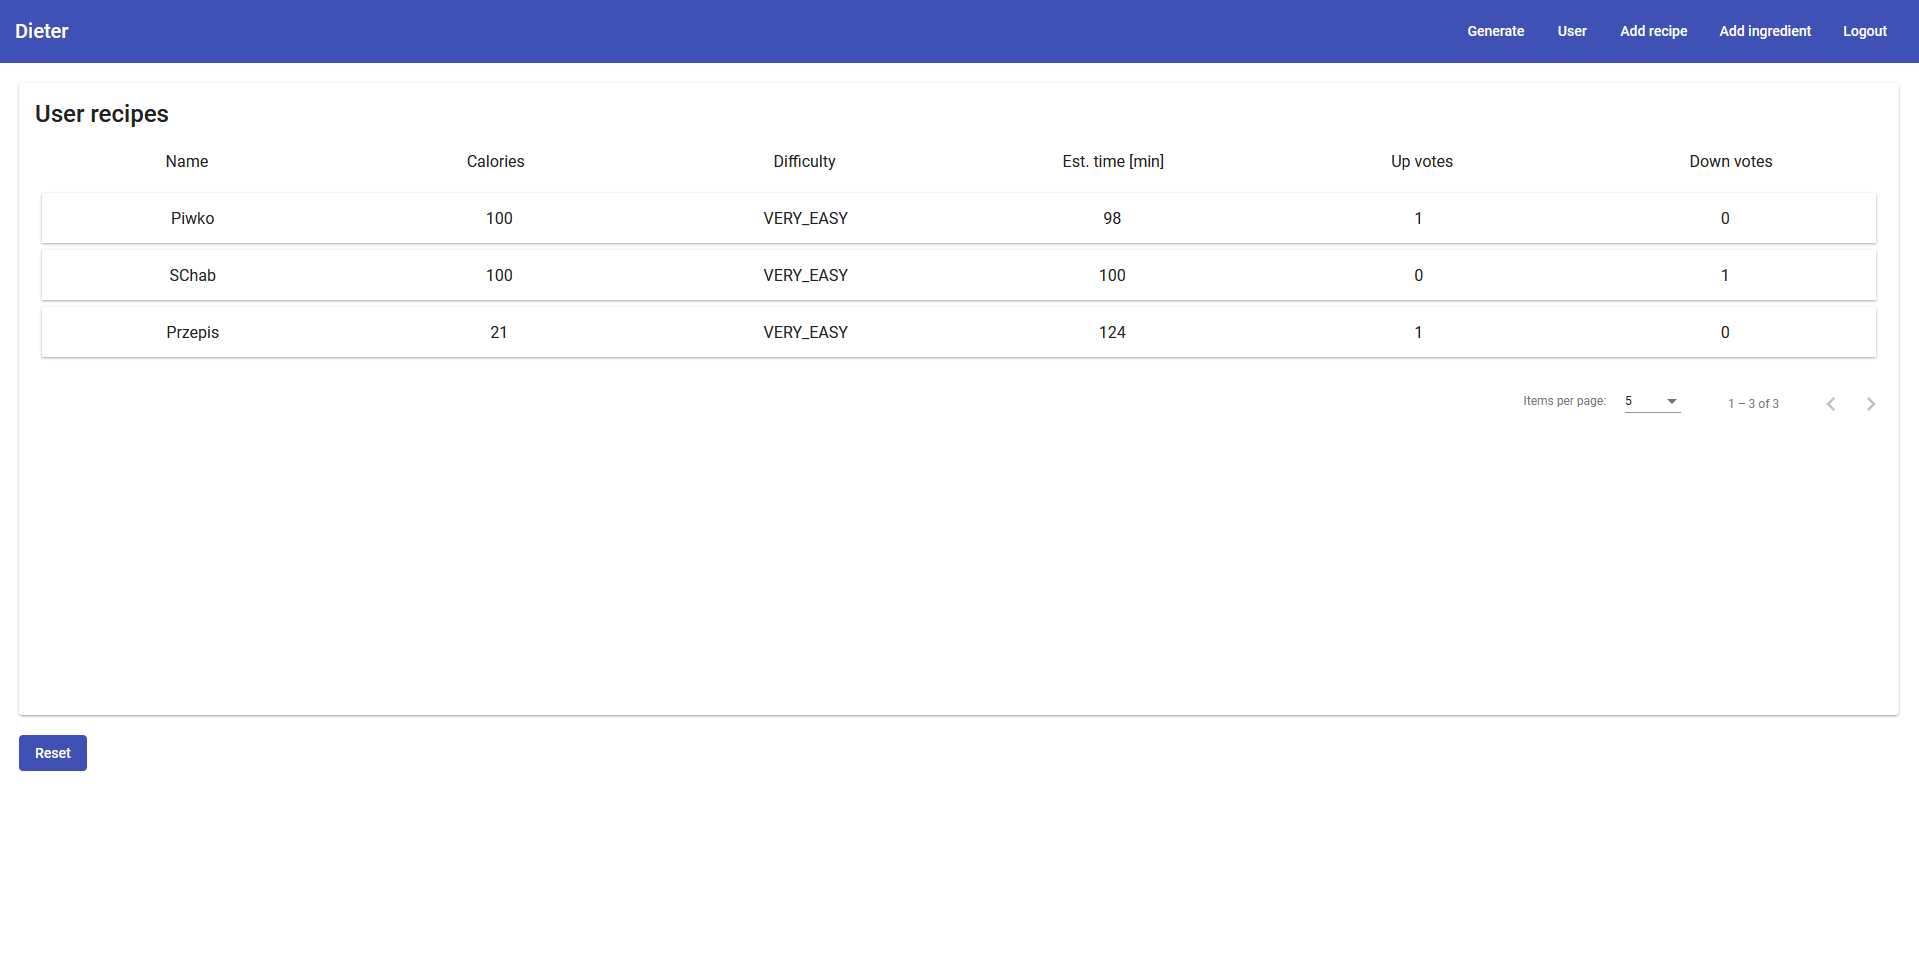
\includegraphics[width=\textwidth]{screeny/generowany.png}
\caption{Wygenerowana dieta}
\label{fig:generowana_dieta}
\end{figure}

\section{Szczegóły użytkownika}
Na Rysunku \ref{fig:user} został pokazany panel szczegółów użytkownika. Widać w nim jego podstawowe informacje oraz listę dodanych przez niego przepisów. Po naciśnięciu w przepisu z listy wyświetlą się jego szczegóły.

\begin{figure}[H]
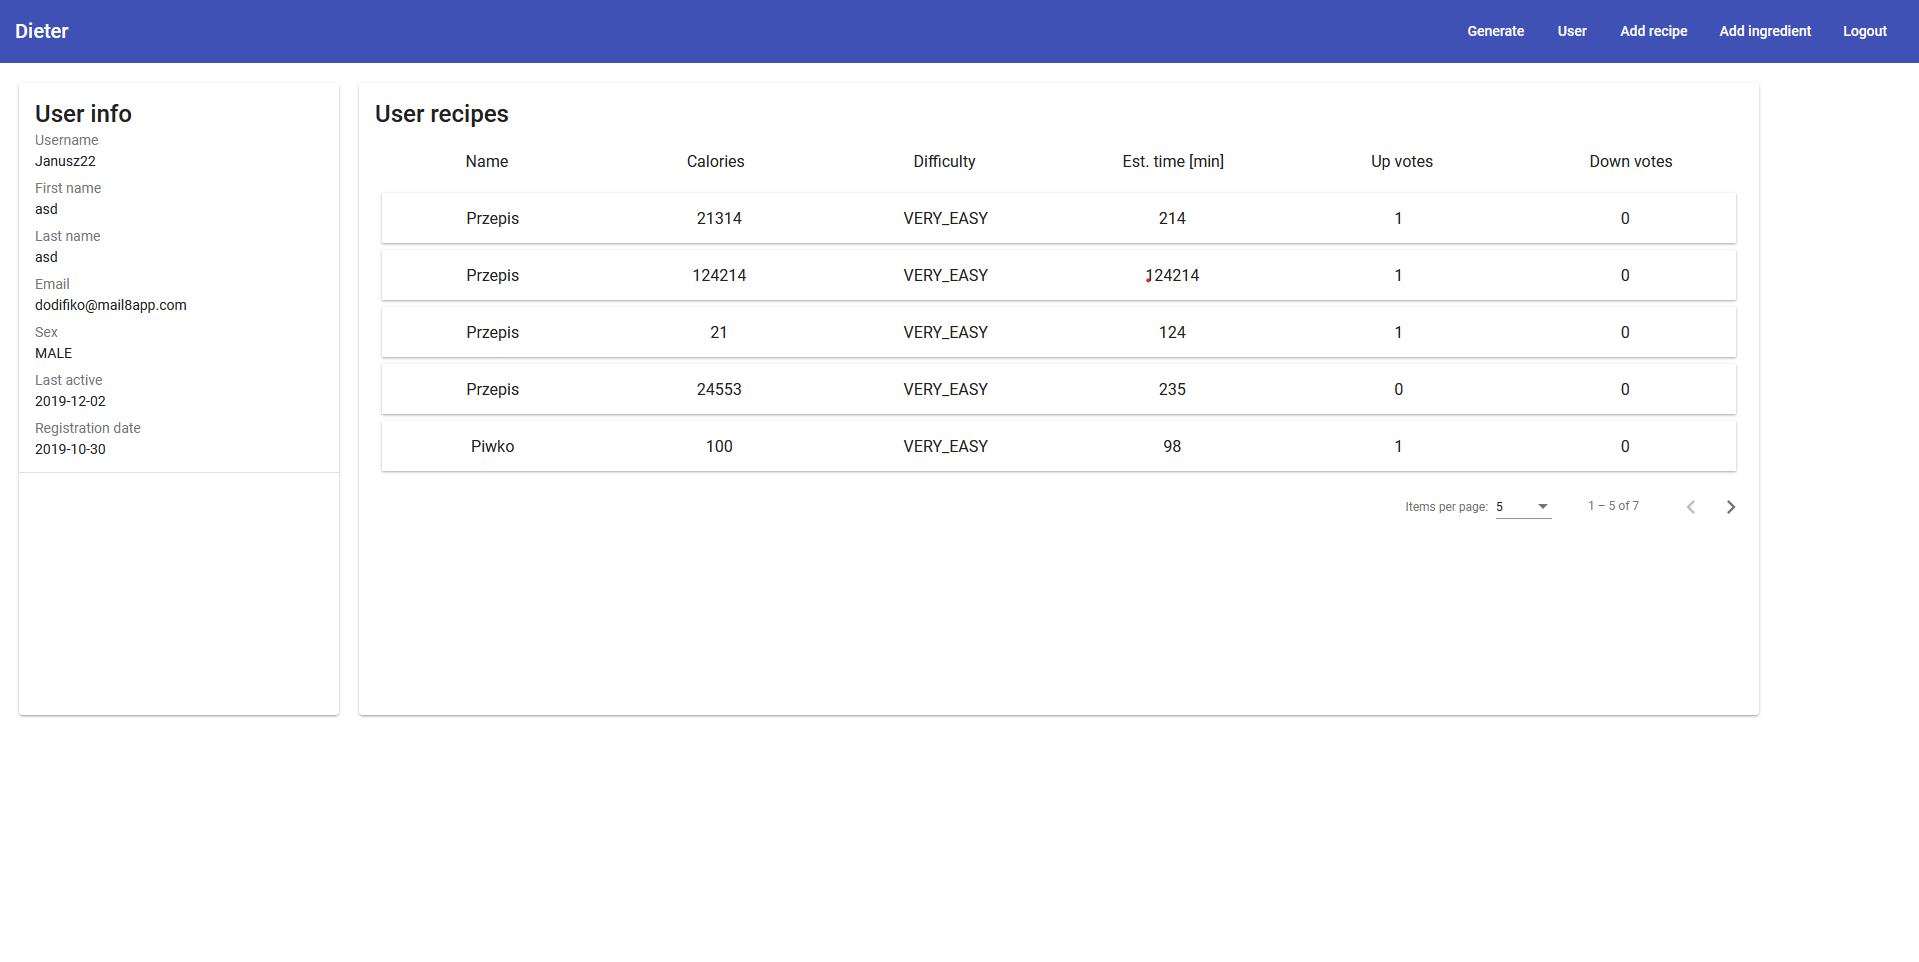
\includegraphics[width=\textwidth]{screeny/user.png}
\caption{Szczegóły użytkownika}
\label{fig:user}
\end{figure}

\section{Dodawanie składnika}
Na Rysunku \ref{fig:ingredient} przedstawiono formularz dodawania składnika. Po wypełnieniu wszystkich wymaganych pól oraz wybraniu kategorii, wystarczy nacisnąć przycisk \textit{Add}.

\begin{figure}[H]
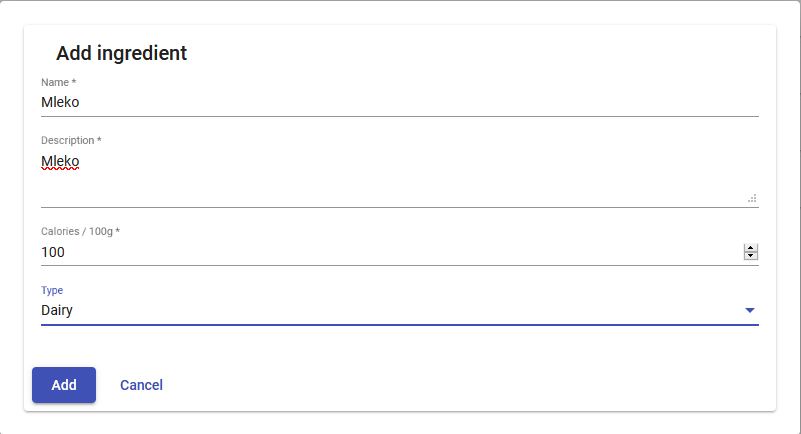
\includegraphics[width=\textwidth]{screeny/dodaj-skladnik.png}
\caption{Dodawanie składnika}
\label{fig:ingredient}
\end{figure}
